
\chapter{Bidirectional Radiance Caching}
\label{chap:bidirectional_caching}

\section{A General Theoretical Framework for Radiance Caching}
Before proposing new radiance caching techniques, I first want to take a step back and analyze radiance caching in general.

Radiance caching generally can be broken down into four steps:

\begin{enumerate}
    \item \textbf{Training}
    \begin{enumerate}
        \item \textbf{Query Prediction} First, we want to predict potential queries $\hat{q} = (\vec{x}, \vec{\omega}_o)$ according to a distribution $\hat{Q}(\hat{q})$.
        \item \textbf{Radiance Estimation} Given a predicted query $\hat{q}$, we want to estimate the outgoing radiance $L_o(\hat{q})$ at that query.
        For this, we can use any possible combination of radiance estimation techniques, such as path tracing, light tracing, photon mapping or bidirectional path tracing (BDPT).
    \end{enumerate}
    \item \textbf{Inference}
    \begin{enumerate}
        \item \textbf{Query Sampling} We sample queries $q = (\vec{x}, \vec{\omega}_o)$ according to a distribution $Q(q)$.
        \item \textbf{Interpolation} Given a query $q$, we want to approximate the outgoing radiance $\hat{L}_o(q)$ by interpolating the radiance estimates of spatiotemporally nearby query predictions $\hat{q}$.
        We can use any combination of storing and interpolation technique for this, such as nearest neighbor, linear interpolation or, in our case, the NRC.
        Note however, that this step generally introduces \textbf{bias}.
    \end{enumerate}
\end{enumerate}

\textbf{Note:} Using this framework we can observe that the \textbf{cache efficiency} is optimal if the query prediction distribution $\hat{Q}(\hat{q})$ is equal to the query sampling distribution $Q(q)$.
Conversely, if we sample a query $q^*$ that can not be predicted by the query predictor (i.e. $\hat{Q}(q^*)=0$), we introduce fundamental bias into the radiance cache $\hat{L}_o(q^*)$, because the radiance cache will not contain an accurate radiance estimate for that query.
This happens, whenever the support of the query sampling distribution $Q$ is not contained in the support of the query prediction distribution $\hat{Q}$, i.e. $\supp(Q) \not\subseteq \supp(\hat{Q})$.

\textbf{Discussion:} It may be possible, to derive a better radiance cache by storing the incoming radiance and BSDFs in a data structure and connecting to them stochastically through ReSTIR DI \bcite{bitterli2020} similar to Virtual Point Lights in Instant Radiosity techniques \bcite{keller1997}.
% Or VCM

The general idea of decoupling radiance estimation and visualization was already explored by others, notably \textcite{walter1999} and \textcite{tole2002}.

\section{The Path Space Integral Formulation}
To be able to robustly derive the following radiance estimators, I will use an alternative but equivalent formulation of the rendering equation as an integral over the path space, which was first introduced by \textcite{veach1997}.
\begin{figure}[ht]
    \centering
    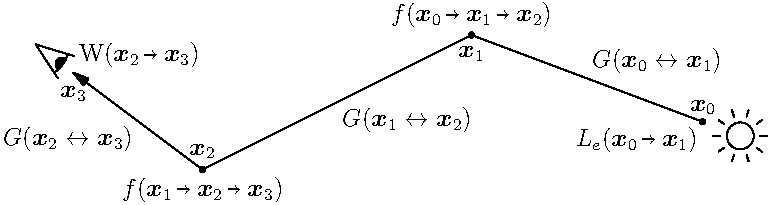
\includegraphics{asy/path_integral.pdf}
\caption{Radiance transfer along a path of length $n=3$ according to the path space integral formulation.}
\label{fig:path_space_integral}
\end{figure}

A path $\bar{x}$ of length $n$ is defined as a sequence of vertices $\vec{x}_0 \vec{x}_1 \dots \vec{x}_n$.
Let the space of all paths of length $n$ be $X_n$ and the space of all paths $X = \bigcup_{n=1}^{\infty} X_n$.
Then, the path space integral formulation of the rendering equation is given by:
\begin{equation}
\label{eq:path_space_integral}
\begin{aligned}
    I
    = \sum_{n=0}^{\infty} \int_{X_n} L_e(\pdir{0}{1}) \G{0}{1} &\prod_{i=1}^{n - 1} \f{i-1}{i}{i+1} \G{i}{i+1}\\
    &\cdot W(\pdir{n-1}{n}) \diff A(\vec{x}_0) \dots \diff A(\vec{x}_n)
\end{aligned}
\end{equation}
To collect incoming radiance at a sensor point $\vec{x}_n$, the path space integral formulation contains a sensor weighting term $W(\pdir{n-1}{n})$, which in the case of an infinitesimal pin-hole camera is simply a Dirac-Delta-function over the eye position and a box function over the viewing directions covered by the pixel.
The arrow notation $\vec{x} \pto \vec{y}$ denotes a ray starting at $\vec{x}$ traveling towards $\vec{y}$, i.e. $L_o(\vec{x} \pto \vec{y}) \defeq L_o(\vec{x}, \vec{y} - \vec{x})$.
The triples represent surface interactions, $f(\vec{x} \pto \vec{y} \pto \vec{z}) \defeq f(\vec{y} - \vec{x}, \vec{y}, \vec{z} - \vec{y})$. 
Double arrow notation is used for path segments, $G(\vec{x} \leftrightarrow \vec{y})$ models the radiance transfer between the vertices $\vec{x}$ and $\vec{y}$:
\begin{equation}
\label{eq:transfer}
G(\vec{x} \leftrightarrow \vec{y}) \defeq V(\vec{x} \leftrightarrow \vec{y}) \frac{\cos \theta_{\vec{x} \veryshortarrow \vec{y}} \cos \theta_{\vec{y} \veryshortarrow \vec{x}}}{\|\vec{y} - \vec{x}\|^2},
\end{equation}
where $V(\vec{x} \leftrightarrow \vec{y}) \in \{0,1\}$ defines visibility and $\theta$ denotes the respective angles of incidence.
The integral is measured over the surface of the scene $A(\vec{x})$.

\begin{figure}[ht]
    \centering
    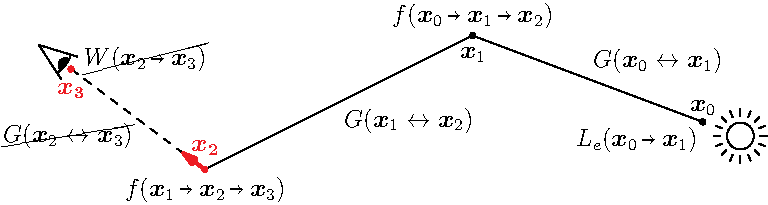
\includegraphics{asy/path_integral_radiance.pdf}
\caption{To estimate the outgoing radiance $L_o(\pdir{2}{3})$ with the path space integral formulation, we fix the last two vertices defining the position and direction, here $\vec{x}_2$ and $\vec{x}_3$ highlighted in red. Furthermore, we drop the sensor weighting term $W$ and the last geometry term $\G{2}{3}$, because they are not part of the path anymore.}
\label{fig:path_space_integral_radiance}
\end{figure}
In the following derivations, I will also use a slightly adapted formulation of the path space integral, that estimates \emph{radiance} instead of \emph{intensity} (see \autoref{fig:path_space_integral_radiance}).
Therefore, we only have to drop the sensor weighting term $W$ and the last geometry term $\G{n-1}{n}$ and fix the last two vertices, which define the position and direction of outgoing radiance, by excluding them from the integration domain:
\begin{equation}
\label{eq:path_space_integral_radiance}
\begin{aligned}
    % L_o(x, \wo) = \sum_{n=0}^{\infty} \int_{X_n} L_e(\pdir{0}{1}) \G{0}{1} \prod_{i=1}^{n - 1} \f{i-1}{i}{i+1} \G{i}{i+1}\\
    % \f{n-1}{n}{} \G{n}{} f(\vec{x}_n \pto \vec{x}, \wo) \ \diff A(\vec{x}_0) \dots \diff A(\vec{x}_n)
    L_o(\pdir{n-1}{n})
    %= L_i(\pdir{n-1}{n})
    = &\sum_{n=0}^{\infty} \int_{X_{n-2}} L_e(\pdir{0}{1}) \\
    &\cdot \prod_{i=1}^{n - 1} \G{i-1}{i} \f{i-1}{i}{i+1} 
    \diff A(\vec{x}_0) \dots \diff A(\vec{x}_{n-2})
\end{aligned}
\end{equation}

The main advantage of these formulations is the independence of the individual vertices.
This for example allows for straightforward bidirectional sampling.
An essential tool for the derivation of path samplers is the conversion between area and solid angle measure, given by:
\begin{equation}
\label{eq:area_solid_angle}
\diff A(\vec{y}) = \frac{\cos \theta_{\vec{y}\veryshortarrow\vec{x}}}{\|\vec{y} - \vec{x}\|^2} \diff \omega(\vec{x}\pto\vec{y}),
\end{equation}
or directly applied to sampling probabilities:
\begin{equation}
\label{eq:area_solid_angle_p}
p(\vec{y}) = \frac{\cos \theta_{\vec{y}\veryshortarrow\vec{x}}}{\|\vec{y} - \vec{x}\|^2} p(\vec{x}\pto\vec{y}).
\end{equation}

\section{Inference}
Using this framework a simple inference scheme naturally emerges from the Path Space Integral Formulation (\autoref{eq:path_space_integral}).
The path length $n$ is limited by a path termination strategy (\autoref{sec:path-termination}), so we only need to calculate the finite sum up to the termination length $l$ because we terminate with a valid radiance estimate which incorporates the sum over longer paths.
We replace the integral over the path space $X_n$ by a primary Monte-Carlo Estimator.
For readability, I will do an exemplary derivation for a path of length $n=2$ without intermediate emission:
\begin{subequations}
\begin{align}
    % Length n=2
    I
    &= \int_{X_n} \widehat{L}_o(\pdir{0}{1}) \G{0}{1} \f{0}{1}{2} \G{1}{2} \cancel{W(\pdir{1}{2})} \diff A(\vec{x}_0) \!\cdots\! \cancel{\diff A(\vec{x}_2)}\notag\\
    &= \int_{X_{n-1}} \widehat{L}_o(\pdir{0}{1}) \G{0}{1} \f{0}{1}{2} \G{1}{2} \diff A(\vec{x}_0) \diff A(\vec{x}_1) \label{eq:cancelw}\\
    &\eqhat \frac{\widehat{L}_o(\pdir{0}{1}) \G{0}{1}}{p(x_0)}  \frac{\f{0}{1}{2} \G{1}{2}}{p(x_1)} \label{eq:pmc}\\
    &= \frac{\widehat{L}_o(\pdir{0}{1}) \cos\theta_{1\veryshortarrow0}}{p(\pdir{1}{0}\mid\pdir{2}{1})}  \frac{\f{0}{1}{2} \cos\theta_{2\veryshortarrow1}}{p(\pdir{2}{1})} \label{eq:area2solid}
    % Length n=3
    % I
    % &= \int_{X_n} \widehat{L}_o(\pdir{0}{1}) \G{0}{1} \f{0}{1}{2} \G{1}{2} \f{1}{2}{3} \G{2}{3} \delta(\pdir{2}{3}) \diff A(\vec{x}_0) \dots \diff A(\vec{x}_3)\\
    % &= \int_{X_{n-1}} \widehat{L}_o(\pdir{0}{1}) \G{0}{1} \f{0}{1}{2} \G{1}{2} \f{1}{2}{3} \G{2}{3} \diff A(\vec{x}_0) \dots \diff A(\vec{x}_2)\\
    % &\approx \frac{\widehat{L}_o(\pdir{0}{1}) \G{0}{1}}{p(x_0)}  \frac{\f{0}{1}{2} \G{1}{2}}{p(x_1)} \frac{\f{1}{2}{3} \G{2}{3}}{p(x_2)}\\
    % &= \frac{\widehat{L}_o(\pdir{0}{1}) \cos\theta_{0\veryshortarrow1}}{p(\pdir{1}{0}\mid\pdir{2}{1})}  \frac{\f{0}{1}{2} \cos\theta_{1\veryshortarrow2}}{p(\pdir{2}{1}\mid\pdir{3}{2})} \frac{\f{1}{2}{3} \cos\theta_{2\veryshortarrow3}}{p(\pdir{3}{2})}\\
\end{align}
\end{subequations}
In the first step, the sensor weighting term $W$ cancels with the integration over the eye vertex (\ref{eq:cancelw}).
We then replace the integral by a primary Monte Carlo estimator (\ref{eq:pmc}).
Finally, we convert from area measure to solid angle measure using (\autoref{eq:area_solid_angle_p}) which cancels with $G$ leaving only the cosine terms at the sampled vertices (\ref{eq:area2solid}).
The visibility term implicitly vanishes in the ray tracing step.
\begin{figure}[ht]
    \centering
    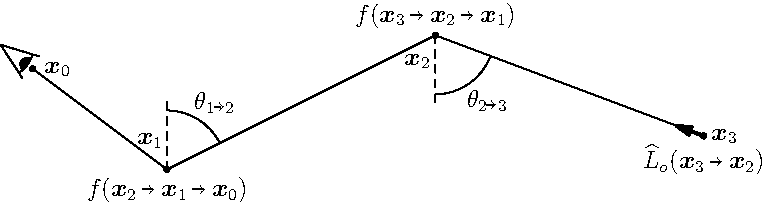
\includegraphics{asy/inference.pdf}
\caption{Visualization of the inference process.}
\label{fig:inference}
\end{figure}

Applying these observations to all path lengths up to termination, we get:
\begin{equation}
\label{eq:inference}
    I
    = \sum_{i=1}^{n-1} T_i L_e(\pdir{i}{i-1}) + T_n \widehat{L}_o(\pdir{n}{n-1}), \quad
    T_n
    = \prod_{i=1}^{n} \frac{f(\ptrip{i-1}{i}{i+1}) \cos \theta_{i \veryshortarrow i+1}}{p(\pdir{i}{i+1} \mid \pdir{i-1}{i})}
\end{equation}
where $T_n$ is the accumulated throughput along the path and $\widehat{L}_o(\pdir{n}{n-1})$ is the interpolated radiance estimate at the termination vertex.
To simplify notation, the path now starts at the eye vertex $\vec{x}_0$.
Note, that Russian Roulette Termination (\autoref{eq:rr}) is not to be applied here, as we terminate the path with a valid radiance estimate.

\section{Path Tracing}

\section{Bidirectional Training}

\section{Light Tracing}

\section{Balancing}

\section{Path Spaced Denoised Sparse Photon Mapping}

%\section{Hardware Accelerated Vertex Connection and Merging}